\documentclass[12pt, a4paper]{article}

%\usepackage[T1,T2A]{fontenc}
\usepackage[utf8]{inputenc}
\usepackage[english,russian]{babel}
\usepackage[left=3cm, right=2cm, top=2cm, bottom=2cm]{geometry}
\usepackage{indentfirst} %Красная строка
\usepackage[shortlabels]{enumitem}
\usepackage{amsmath} %фигурная скобка
\usepackage{autonum}
\usepackage{multicol, multirow}
\usepackage{csvsimple}
\usepackage{graphicx}
\graphicspath{{noiseimages/}}

\usepackage{caption}
\captionsetup{labelsep=endash}
\captionsetup[figure]{name={Рисунок}}


\usepackage{listings} %вставка кода

\usepackage{xcolor}
\definecolor{darkgray}{gray}{0.15}
\lstset{ % add your own preferences
	frame=single,
	basicstyle=\footnotesize\ttfamily,
	identifierstyle=\color{darkgray},
	keywordstyle=\color{black},
	numbers=left,
	numbersep=10pt,
	stepnumber=1,
	numberstyle=\tiny,
	showstringspaces=false, 
	captionpos=t,
	tabsize=4,
	language=Python
}

\usepackage{titlesec}
\titlespacing*{\subsection}{\parindent}{*4}{*4}

\linespread{1.25} %межстрочный интервал
\newcommand{\anonsection}[1]{ \section*{#1} \addcontentsline{toc}{section}{\numberline {}#1}}


\begin{document}
	\lstset{language=Python}
	\section*{Введение}
	Целью лаборатоной работы является изучение и реализация алгоритмов нахождения расстояний
	Левенштейна и Дамерлау-Левештейна, а также получения навыка динамического программирования. Для её достижения необходимо выполнить следующие задачи:
	\begin{itemize}
		\item Изучение алгоритмов Левенштейна и Дамерлау-Левештейна
		\item Разработать данные алгоритмы
		\item Применение методов динамического программирования для реализации алгоритмов
		\item Выполнить тестирование реализации алгоритмов методом черного ящика
		\item Провести сравнительный анализ этих алгоритмов по затратам памяти и процессорному выполнению времени на основе экспериментальных данных
	\end{itemize}

	\newpage
	\section{Аналитический раздел}
		\subsection{Расстояние Левенштейна}
		Расстояние Левенштейна (редакторское расстояние) между двумя строками [1] - минимальное количество
		операций вставки, удаления и замены, необходимых для превращения одной строки в другую.\\
		При преобразовании одной строки в другую, используются следующие операции:
		\begin{enumerate}[a)]
			\item I (insert) - вставка;
			\item D (delete) - удаление;
			\item R (replace) - замена; 
		\end{enumerate}
		Будем считать, что стоимость каждой из этих операции (штраф) равна 1.\\
		Введем еще одну операцию M (match) - совпадение. Её стоимость будет равна нулю.
		Необходимо найти последовательность замен с минимальным суммарным штрафом.
		
		\subsection{Рекурсивный алгоритм}
		Расстояние между двумя строками s1 и s2 рассчитывается по реккуретной формуле D:
		$$
			D(s1[1..i], s2[1..j]) = 
			\begin{cases}
				0, \quad \phantom{\infty}\text{i=0, j=0}\\
				j, \quad \phantom{\infty}\text{i=0, j>0}\\
				i, \quad \phantom{\infty}\text{i>0, j=0}\\
				\min \begin{cases}
					 D(s1[1..i], s2[1..j-1]) + 1\\
					 D(s1[1..i-1], s2[1..j]) + 1\\
					 D(s1[1..i-1], s2[1..j-1]) + f(s1, s2)\\
					 \end{cases}
			\end{cases}
			\label{eq}
			\eqno(1.2.1)
		$$
		Функция f(s1, s2) определяется следующим образом:
		$$
			f(s1, s2) =
			\begin{cases}
				0, \text{  s1=s2}\\
				1, \text{  иначе}
			\end{cases}
			\eqno(1.2.2)
		$$
		
		\subsection{Матрица расстояний}
		Реализация формулы 1.2.1 при больших значениях i,j, оказывается менее эффективной по времени ввиду того, что приходится вычислять промежуточные результаты неоднократно. Для оптимизации нахождения расстояния Левенштейна необходимо использовать матрицу стоимостей для хранения этих промежуточных значений. Таким образом, будет необходимо выполнять только построчное заполнение такой матрицы.
		
		\subsection{Рекурсивный алгоритм с кэшем в форме матрицы}
		При помощи использования матрицы можно выполнить оптимизацию рекурсивного алгоритма заполнения. Основная идея такого подхода заключается в том, что при каждом рекурсивном вызове алгоритма выполняется заполнение матрицы стоимостей. Главное отличие данного метода от того, что был описан в разделе 2.3 - начальная инициализация матрицы флагом $\infty$. То есть если рекурсивный алгоритм выполняет прогон для данных, которые не были обработаны, результат заносится в матрицу. Если же используются повторные данные (ячейка матрицы была заполнена), то алгоритм не выполняет вычисление расстояния для этой ячейки, а сразу переходит к следующему шагу.
		
		\subsection{Расстояние Дамерау-Левенштейна}
		Расстояние Дамерау-Левенштейна является модификацией расстояния Левенштейна, которая задействует еще одну редакторскую операцию - транспозицию T
		(transposition. Она выполняет обмен соседних символов в слове. \\
		Дамерау показал, что 80\% человеческих ошибок при наборе текстов является перестановка соседних символов, пропуск символа, добавление нового символа или ошибочный символ. Таким образом, расстояние Дамерау-Левенштейна часто используется в редакторских программах для проверки правописания.
		Это расстояние может быть вычислено по следующей реккуретной формуле:
		 $$
		 D(s1[1..i], s2[1..j]) = 
		 \begin{cases}
		 	0, \quad \phantom{\infty}\text{i=0, j=0}\\
		 	j, \quad \phantom{\infty}\text{i=0, j>0}\\
		 	i, \quad \phantom{\infty}\text{i>0, j=0}\\
		 	\min \begin{cases}
		 		D(s1[1..i], s2[1..j-1]) + 1\\
		 		D(s1[1..i-1], s2[1..j]) + 1\\
		 		D(s1[1..i-1], s2[1..j-1]) + f(s1, s2)\\
		 		D(s1[1..i-1], s2[1..j-1]) + 1, \text{   i,j > 1$,a_{i}=b_{j-1},$ $a_{i-1}=b_{j}$}\\
		 		{\infty},\text{      иначе}\\
		 	\end{cases}\\
	 		
		 \end{cases}
		 \label{eq}
		 \eqno(1.5.1)
		 $$
		 
		 \subsection{Вывод}
		 В данном разделе были рассмотрены основные способы нахождения редакторского расстояния между двумя строками. Формулы для нахождения расстояния Левенштейна и Дамерау-Левенштейна задаются реккуретно, следовательно, алгоритмы могут быть реализованы как рекурсивно, так и итерационно.
		 
	\newpage
	\section{Конструкторская часть}
	\subsection{Схемы алгоритмов Левенштейна}
	рис \ref{png:1} - схема алгоритма итеративного алгоритма Левенштейна с использованием двух строк
	рис \ref{png:2} - схема алгоритма рекурсивного алгоритма Левенштейна без кэша
	рис \ref{png:3} - схема алгоритма рекурсивного алгоритма Дамерау-Левенштейна с использованием матрицы
	
	\subsection{Схема алгоритма Дамерау-Левенштейна}
	рис \ref{png:5} - схема алгоритма итеративного алгоритма Левенштейна с использованием двух строк
	
	\begin{figure}[pht!]
		\centering{
			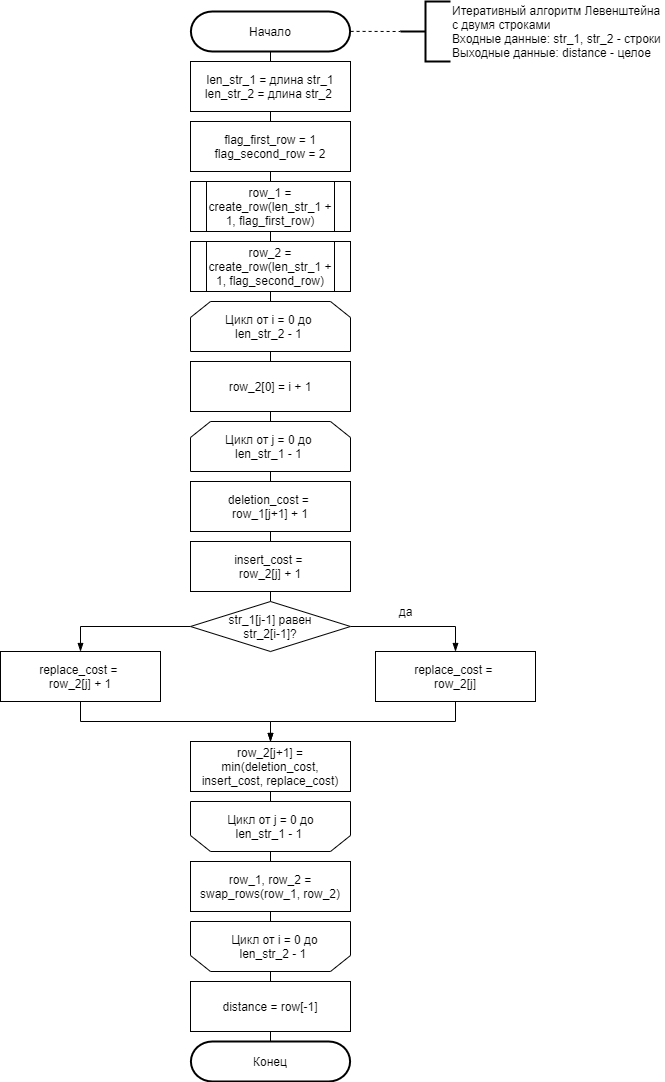
\includegraphics[width=14.6cm]{../../../../../../../msys64/home/Лев/bmstu_sem_5_aa/lab_01/report/diagrams/iterative_two_rows}
			\caption{Сравнение времени работы алгоритмов Левенштейна.}
			\label{png:1}}
	\end{figure} 

	\begin{figure}[pht!]
		\centering{
			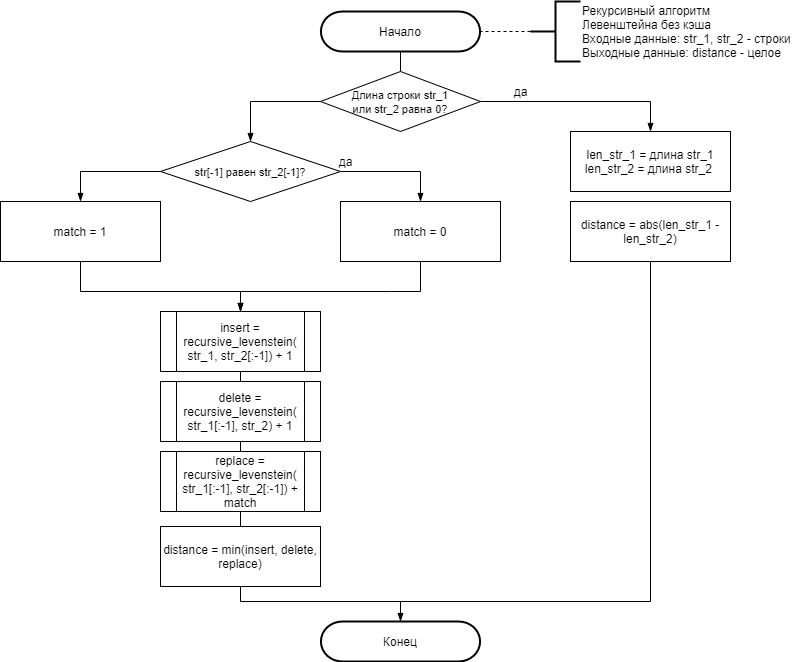
\includegraphics[width=14.6cm]{../../../../../../../msys64/home/Лев/bmstu_sem_5_aa/lab_01/report/diagrams/Рекурсивный Левенштейн без кэша}
			\caption{Сравнение времени работы алгоритмов Левенштейна.}
			\label{png:2}}
	\end{figure} 

	\begin{figure}[pht!]
		\centering{
			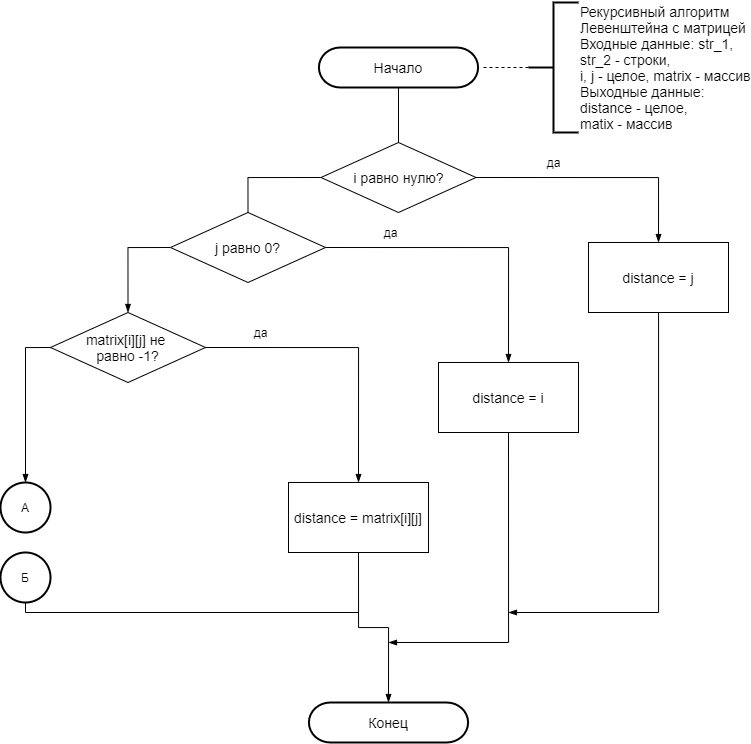
\includegraphics[width=14.6cm]{../../../../../../../msys64/home/Лев/bmstu_sem_5_aa/lab_01/report/diagrams/Рекурсивный Левенштейн с матрицей1}
			\caption{Сравнение времени работы алгоритмов Левенштейна.}
			\label{png:3}}
	\end{figure}

	\begin{figure}[pht!]
		\centering{
			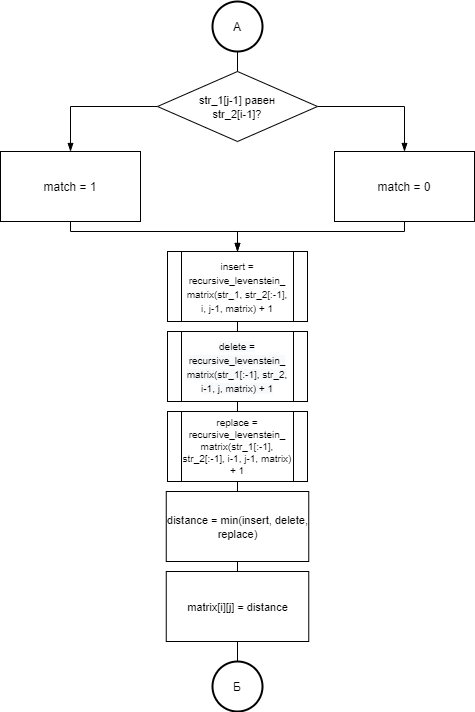
\includegraphics[width=14.6cm]{../../../../../../../msys64/home/Лев/bmstu_sem_5_aa/lab_01/report/diagrams/Рекурсивный Левенштейн с матрицей2}
			\caption{Сравнение времени работы алгоритмов Левенштейна.}
			\label{png:4}}
	\end{figure}  
	\newpage

	\begin{figure}[pht!]
		\centering{
			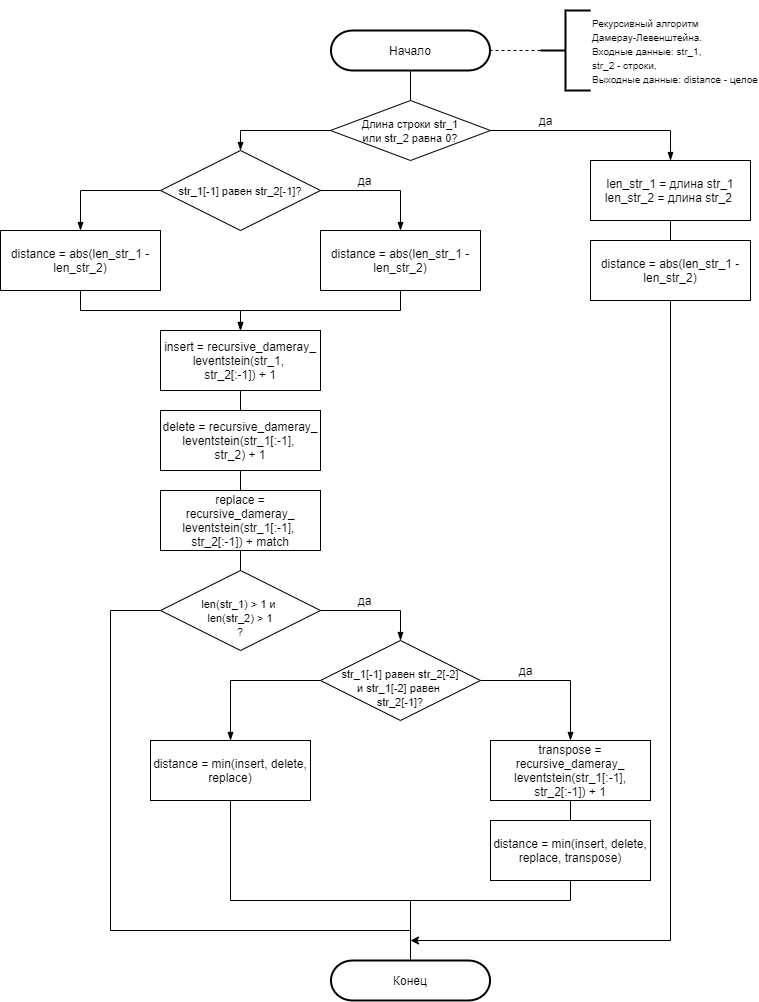
\includegraphics[width=14.6cm]{../../../../../../../msys64/home/Лев/bmstu_sem_5_aa/lab_01/report/diagrams/Рекурсивный Дамерау-Левенштейн}
			\caption{Сравнение времени работы алгоритмов Левенштейна.}
			\label{png:5}}
	\end{figure} 
	
\newpage
\section{Технологическая часть}
\subsection{Требования к программному обеспечению}
Программа должна отвечать следующим требованиям:
\begin{itemize}
	\item На вход программе подаются две строки на русском или английском языке в любом регистре;
	\item Осуществляется выбор алгоритма нахождения расстояния из меню
	\item На выходе программа выдает результат - найденное расстояние между двумя строками выбранным пользователем алгоритмом
\end{itemize}
\subsection{Выбор средств реализации}
Для реализации алгоритмов в данной лабораторной работе был выбран язык программирования python. Он является кроссплатформенный, а также имеется опыт разработки на этом языке. В качестве среды разработки был использован Visual Studio Code, так как в нем можно работать как на операционной системе Windows, так и на дистрибутивах Linux. При замере процессорного времени был использован модуль ***.
\subsection{Листинги программ}
\begin{lstlisting}[label=some-code,caption=Программный код нахождения расстояния Левенштейна итеративно с использованием двух строк]
	def iterative_levenstein_two_rows(str_1: str, str_2: str) -> int:
	len_str_1 = len(str_1); len_str_2 = len(str_2)
	flag_first_row = 1; flag_second_row = 2
	
	row_1 = create_row(len_str_1 + 1, flag_first_row)
	row_2 = create_row(len_str_1 + 1, flag_second_row)
	
	for i in range(len_str_2):
	row_2[0] = i + 1
	for j in range(len_str_1):
	deletion_cost = row_1[j + 1] + 1
	insert_cost = row_2[j] + 1
	replace_cost = row_1[j] if str_1[j - 1] == str_2[i - 1] \
	else row_1[j] + 1
	
	row_2[j + 1] = min(deletion_cost, insert_cost, replace_cost)
	row_1, row_2 = swap_rows(row_1, row_2)
	distance = row_1[-1]
	return distance
\end{lstlisting}

\begin{lstlisting}[label=some-code,caption=Программный код нахождения расстояния Левенштейна рекурсивно без использования кэша]
	def recursive_levenstein(str_1: str, str_2: str) -> int:
	if str_1 == '' or str_2 == '':
	return abs(len(str_1) - len(str_2))
	match = 0 if str_1[-1] == str_2[-1] else 1
	distance = min(recursive_levenstein(str_1, str_2[:-1]) + 1,
	recursive_levenstein(str_1[:-1], str_2) + 1,
	recursive_levenstein(str_1[:-1], str_2[:-1]) + match)
	return distance
\end{lstlisting}

\begin{lstlisting}[label=some-code,caption=Программный код нахождения расстояния Левенштейна рекурсивно с использованием матрицы]
	def recursive_levenstein_matrix(str_1: str, str_2: str, i: int, j: int,
	matrix: list) -> Tuple[int, list[list[int]]]:
	if i == 0:
	return j, matrix
	if j == 0:
	return i, matrix
	if matrix[i][j] != -1:
	return matrix[i][j], matrix
	match = 0 if str_1[-1] == str_2[-1] else 1
	
	insert, matrix = recursive_levenstein_matrix(str_1, str_2[:-1], i,
	j-1, matrix)
	delete, matrix = recursive_levenstein_matrix(str_1[:-1], str_2, i-1,
	j, matrix)
	replace, matrix = recursive_levenstein_matrix(str_1[:-1], str_2[:-1],
	-1, j-1, matrix)
	insert += 1; delete += 1; replace += match
	
	distance = min(insert, delete, replace)
	matrix[i][j] = distance
	return distance, matrix
\end{lstlisting}

\begin{lstlisting}[label=some-code,caption=Программный код нахождения расстояния Дамерау-Левенштейна рекурсивно]
	def recursive_dameray_levenstein(str_1: str, str_2: str) -> int:
	if str_1 == '' or str_2 == '':
	return abs(len(str_1) - len(str_2))
	match = 0 if str_1[-1] == str_2[-1] else 1
	insert = recursive_dameray_levenstein(str_1, str_2[:-1]) + 1
	delete = recursive_dameray_levenstein(str_1[:-1], str_2) + 1
	replace = recursive_dameray_levenstein(str_1[:-1], str_2[:-1]) + \
	match
	
	if len(str_1) > 1 and len(str_2) > 1 and str_1[-1] == str_2[-2] \
	and str_2[-1] == str_1[-2]:
	distance = min(insert, delete, replace,
	recursive_dameray_levenstein(str_1[:-2], str_2[:-2]) + 1)
	else:
	distance = min(insert, delete, replace)
	return distance
\end{lstlisting}

\Large Утилиты \\
\normalsize На листингах представлены программные модули, которые используются в данных функциях:\\
\begin{lstlisting}[label=some-code,caption=Программный код создания для кэша в виде строки]
	def create_row(len_row: int, flag_row: int) -> list[int]:
	row = list()
	if flag_row == 1:
	for i in range(len_row):
	row.append(i)
	else:
	for i in range(len_row):
	row.append(0)
	return row
\end{lstlisting}

\begin{lstlisting}[label=some-code,caption=Программный код создания для кэша в виде строки]
	def swap_rows(row_1: list[int], row_2: list[int]) \
	-> Tuple[list[int], list[int]]:
	temp_row = list()
	temp_row = deepcopy(row_1)
	row_1 = deepcopy(row_2)
	row_2 = deepcopy(temp_row)
	return row_1, row_2
\end{lstlisting}

\subsection{Тестирование}
Для тестирования используется метод черного ящика. В данном разделе приведена таблица \ref{table:ref1}, в которой указаны классы эквивалентностей тестов \\

\begin{table}[ht!]
	\centering
	\caption{Таблица тестов}
	\label{table:ref1}
	\begin{tabular}{|c|c|c|c|c|c|}
		\hline
		\multirow{3}{*}{№} & \multirow{3}{*}{Описание теста} & \multirow{3}{*}{Слово 1}  &  \multirow{3}{*}{Слово 2}   & \multicolumn{2}{|c|}{Алгоритм}\\ \cline{5-6}
		&                &          &            &\multirow{2}{*}{Левенштейн}   &Дамерау-	\\ 
		&                &          &            &             &Левенштейн       	        \\ \hline
		1& Пустые строки  &  ''      &    ''      &   0         &  0 						\\ \hline
		2& Нет повторяющихся символов & deepcopy & раздел & 8   &  8                       \\ \hline
		3& Инверсия строк & insert   &tresni      &   6         &  6                       \\ \hline
		4& Два соседних символа       & heart    & heatr  & 2   &  1                       \\ \hline
		5& Одинаковые строки          & таблица  & таблица& 0   &  0						\\ \hline
		6& Одна строка меньше другой  & город    & горо   & 1   &  1						\\ \hline
	\end{tabular}
\end{table}

\subsection{Вывод}
В данном разделе был выбран язык программирования, среда разработки. Реализованы функции, описанные в аналитическом разделе, и проведено их тестирование методом черного ящика по таблице \ref{table:ref1}. 


\newpage
\section{Исследовательская часть}
\subsection{Технические характеристики}
Технические характеристии устройства, на котором выполнялось тестирование:
\begin{itemize}
	\item Операционная система: Windows 10 Pro
	\item Память: 8 GiB
	\item Процессор: Intel(R) Core(TM) i5-8265U CPU @ 1.60GHz   1.80 GHz
\end{itemize}
Тестирование проводилось на ноутбуке, который был подключен к сети питания. Во время проведения тестирования ноутбук был нагружен только встроенными приложениями окружения, самим окружением и системой тестирования

\subsection{Временные харастеристики выполнения}
Замер процессорного времени работы алгоритмов производилось при помощи модуля time функцией process\_time().
Проведем анализ времени работы алгоритмов. Исходными данными будут случайно сгенерированные строки длиной {3, 4, 5, 6, 7, 8}. Единичные замеры выдадут крайне маленький результат, поэтому  проведем работу каждого алгоритма n = 1000 раз и поделим на число n. Получим среднее значение работы каждого из алгоритмов. Результат приведен на рис \ref{fg:ref1}:

\begin{figure}[ht!]
	\centering{
		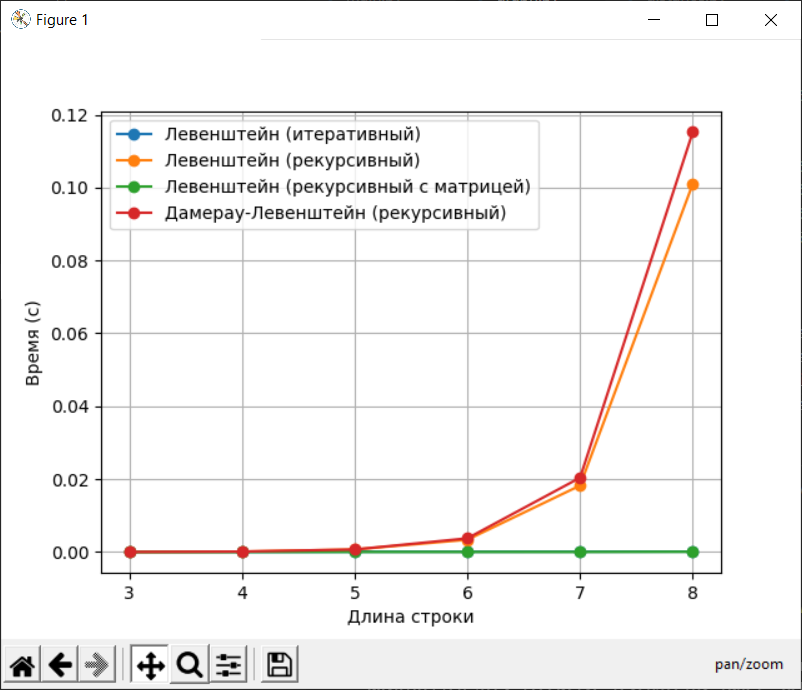
\includegraphics[width=10.6cm]{../../../../../../../msys64/home/Лев/bmstu_sem_5_aa/lab_01/report/image/graph}
		\caption{Сравнение времени работы алгоритмов Левенштейна.}
		\label{fg:ref1}}
\end{figure} 

Как видно из результатов, рекурсивный алгоритм Левенштейна без кэша и алгоритм Дамерау-Левенштейн имеют большой асимпотический рост, начиная уже со строки длиной 7. Последний имеет наибольший рост. Это объясняется тем, что этот алгоритм задействует дополнительную операцию - транспонирование, которая тоже приводит к вызову рекурсии. \\
Выполнив анализ двух остальных алгоритмов на значения входных строк длиной {25, 50, 75, 100, 125, 150}, получим слежующий результат, представленный на рис \ref{fg:ref2}:
\begin{figure}[ht!]
	\centering{
		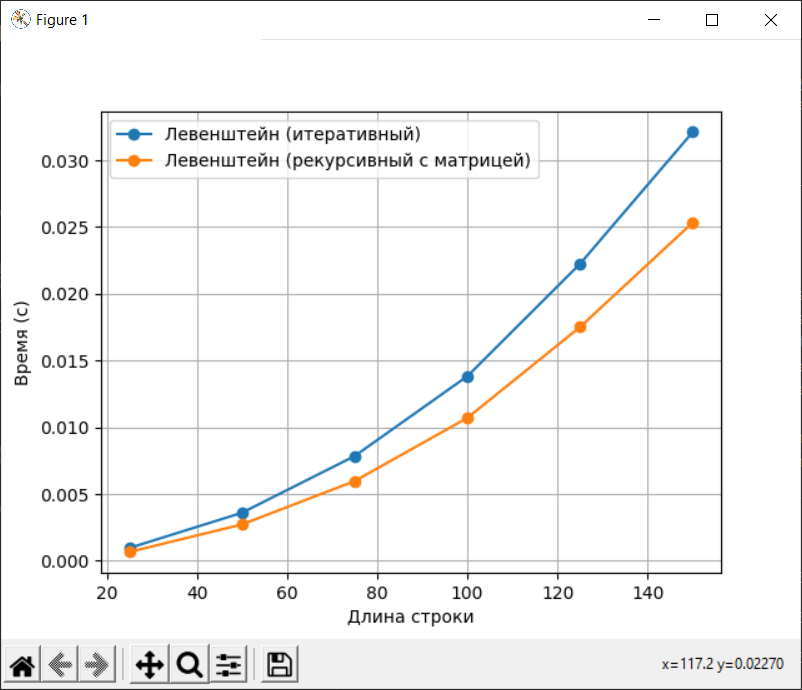
\includegraphics[width=10.6cm]{../../../../../../../msys64/home/Лев/bmstu_sem_5_aa/lab_01/report/image/graph_2}
		\caption{Сравнение времени работы рекурсивного и некурсивного алгоритмов Левенштейна.}
		\label{fg:ref2}}
\end{figure} 

Рекурсивный алгоритм Левенштейна с использованием матрицы выполняется быстрее, нежели чем итеративный с использованием двух строк. Это объясняется тем, что в итеративном случае выполняется дополнительная операция по обмену значений двух строк. На это необходимо дополнительное время.

\subsection{Объем потребляемой памяти}
Замеры используемой памяти и число вызовов рекурсии проводились при помощи модуля memory\_profiler. При исходных строках, длинною 3, требуется 52,8 Mb памяти. Результаты вызовов и объем потребляемой памяти приведены в таблице \ref{table:ref2}:
\begin{table}[ht!]
	\centering
	\caption{Число вызовов каждого алгоритма}
	\label{table:ref2}
	\begin{tabular}{|c|c|c|c|}
		\hline
		\multicolumn{3}{|c|}{Левенштейн} & Дамерау-Левенштейн \\ \cline{1-3} 
		\hline
		\multirow{2}{*}{Итеративный} &\multirow{2}{*}{Рекурсивный} & \multirow{2}{*}{Рекурсивный} & \multirow{2}{*}{Рекурсивный} \\
		с двумя строками & без кэша  & с матрицей & \\
		\hline
		1 & 94 & 28 & 94 \\ 
		\hline
	\end{tabular}
\end{table}\\
\\
Общее значение потребляемой памяти складывается по формуле \ref{eq:2}:
$$
S = n\_calls * V
\label{eq:2}
\eqno(4.3.1)
$$
где:
\begin{itemize}
	\item n\_calls - число вызовов функций
	\item V - объем памяти, занимаемый одним вызовом функции
\end{itemize}
По результатам исследования памяти алгоритм Левенштейна и Дамерау-Левенштейна потребляют больше всего памяти при работе. Итеративный алгоритм Левенштейна с двумя строками занимает меньше всего памяти

\subsection{Вывод}
Приведенные в разделах (4.2) и (4.3) характеристики позволяют сделать вывод о том, что рекурсивный вызов Левенштейна без кэша и Дамерау-Лвенштейна проигрывают как по скорости, так и по памяти итеративному. Причем рекурсивный алгоритм Левенштейна с матрицей работает быстрее, чем итеративный с двумя строками, но также проигрывает ему по памяти.\\
Сравнивая между собой рекурсивные вызовы алгоритмов Левенштейна и Дамерау-Левенштейна, можно сделать вывод о том, что рекурретный алгоритм поиска расстояния Левенштейна с матрицей выигрывает как по времени, так и по памяти, а рекуррентный Дамерау-Левенштейн проигрывает по обоим параметрам. Однако, стоит отметить, что в системах автоматического исправления текста, где чаще всего встречаются ошибки, связанные с транспозицией двух символов, алгоритм Дамерау-Левенштейна будет наиболее оптимальным.\\

\end{document}